\section{Design of the archived numerical studies}
\label{sec:expanded-design}
We now describe the computational studies in enough detail
to distinguish a statistically meaningful result from a
mere timing difference. Experiments were performed
before figure rendering and their original CSVs are
reused verbatim.

\subsection{Full-factorial backend and search comparison}
The author's Windows full-factorial experiment contains
80,640 recorded search records, not 80,640 statistically
independent series. It crosses $n\in\{24,48\}$,
orders $d=0,\ldots,5$, fixed reference means
$\mu\in\{0,0.15\}$, five scores (CV, GCV,
AICc, BIC and conditional Gaussian MLE),
seven backends, and $R\in\{1,3,8\}$ independent
series per workload with cold and shared preparation.
Two seeds, seven timing repetitions and one
BLAS thread were used. The archived environment
records Windows, Python 3.11, NumPy 2.4.6,
SciPy 1.17.1 and the OpenBLAS version.

The reference grid has seventeen $S$ targets:
the deciles between 0 and 1, plus six values
concentrated in the near-one tail from $0.95$
through $1-10^{-12}$. The exact endpoints
are analytic; CV/GCV at the $S=0$
interpolating limit need not admit a finite
ordinary value, and Gaussian marginal MLE
at $d=0$ is not applicable under the adopted model.
A computational record failing parity with the
spectral score is identified as invalid, not
allowed to win because its measured runtime
happened to be short.

There are five \emph{selection} policies of interest:
(i) full-grid native-$S$ search with an inverse
at each candidate; (ii) one-time mapped-$S$
penalty grid followed by $\lambda$-based search;
(iii) a direct finite log-$\lambda$ grid;
(iv) bounded local continuous optimization in
$S$; and (v) bounded local continuous optimization
in $\log\lambda$. The first two evaluate
\emph{identical} candidates; the third does
not, and the two continuous searches use a
variable number of objective evaluations.
Local continuous minima are \emph{not} evidence
of global optimality.

\subsection{Independent-seed solver inference}
A second author-run Windows study measures
preparation plus $M$ complete fitted curves
rather than a scalar trace or criterion.
It uses 20 independently seeded data sets
per predeclared workload and five randomized
technical timing blocks per seed.
For each paired solver comparison, let
$t_{a,i}$ and $t_{b,i}$ be the median full-task
times over timing blocks for data seed $i$.
The primary effect is a geometric mean time ratio
\[
R_{a/b}=\exp\left[
  \frac1N\sum_{i=1}^N\log
  \left(\frac{t_{a,i}}{t_{b,i}}\right)
\right].
\]
Values above one favor the denominator method.
Pointwise 95\% percentile bootstrap intervals
resample data seeds; two-sided paired sign-flip
tests are Holm-adjusted across the predeclared
comparison family. The same-host timing blocks
and the $M$ fitted penalties are \emph{not}
independent inferential units.
Sign-flip inference relies on the exchangeability/
symmetry assumption for paired log differences,
and all conclusions remain conditional on the
recorded hardware and software environment.

\subsection{Four root finders in float64}
The inversion experiment examines Brent, bracket-
safeguarded Newton, bracket-safeguarded secant and
bisection with $n=30,60,120$, $d=0,1,2,3$,
eleven targets from $10^{-14}$ to $1-10^{-14}$,
and 35 randomized timing blocks per method and
target. Every method receives the \emph{same}
already prepared smoothness spectrum.
Outcomes include successful latency, convergence
failure, iterations, function and derivative
evaluations, and tail accuracy. The $d=0$
analytic identity-spectrum inverse is recorded
but excluded from numerical-root comparisons.
These are technical timing replicates on one
host, not 35 independent data sets; accordingly
they do not receive artificial inferential
$p$ values.

\section{Computational results}\label{sec:expanded-results}
\subsection{Grid coordinate, method and reference mean}
Table~\ref{tab:expanded-coordinates} reproduces
the recorded Windows subset at $n=48$,
$d=2$, $R=1$, SVD, comparing every
selection criterion and both fixed reference
means. The reported unit is milliseconds.
The native-$S$ and premapped-$S$ searches
select exactly the same $S$ values because
the finite candidate set is identical.
In contrast, the independently sampled
log-penalty grid changes interior candidates
and occasionally changes the selected value.
Its lower runtime therefore does \emph{not}
establish a better way to find the same
finite-grid statistical estimator.

\begin{table}[tbp]
\centering\scriptsize
\caption{Recorded 17-point Windows complete-search
timings (ms), fixed $n=48,d=2,R=1$, spectral
SVD, two seeds. The first two policies share
all penalty candidates; log-$\lambda$ has
different interior candidates. The final column
shows its selected normalized smoothness and is
included to make non-equivalence visible.
Only numerically valid archive records appear.}
\label{tab:expanded-coordinates}
\resizebox{\linewidth}{!}{\begin{tabular}{llrrrrr}
\toprule
Fixed $\mu$ & Criterion & $S_{\mathrm{native}}$ & Native $S$ & Mapped $\lambda$ & Log-$\lambda$ & $S_{\log\lambda}$ \\
\midrule
0.00 & CV & 0.850 & 2.004 & 1.879 & 0.545 & 0.887 \\
0.00 & GCV & 0.850 & 1.851 & 1.800 & 0.426 & 0.887 \\
0.00 & AICc & 0.900 & 1.887 & 1.810 & 0.458 & 0.887 \\
0.00 & BIC & 0.100 & 2.016 & 1.810 & 0.449 & 0.100 \\
0.00 & MLE & 0.800 & 3.477 & 2.035 & 0.515 & 0.818 \\
0.15 & CV & 0.750 & 1.962 & 1.869 & 0.580 & 0.750 \\
0.15 & GCV & 0.750 & 1.933 & 1.765 & 0.432 & 0.750 \\
0.15 & AICc & 0.800 & 1.876 & 1.781 & 0.439 & 0.750 \\
0.15 & BIC & 0.100 & 1.909 & 1.791 & 0.464 & 0.100 \\
0.15 & MLE & 0.550 & 2.033 & 1.850 & 0.525 & 0.458 \\
\bottomrule
\end{tabular}
}
\end{table}

\begin{figure}[tbp]
\centering
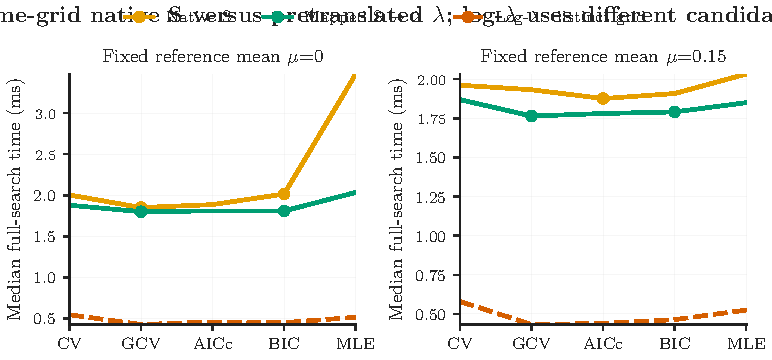
\includegraphics[width=\linewidth]{figures/sncs_coordinate_methods.pdf}
\caption{Recorded end-to-end selection time for
each criterion under $\mu=0$ and $\mu=0.15$.
Native $S$ and premapped $S\to\lambda$
operate on the same seventeen candidates.
The distinct log-$\lambda$ grid is shown
as a timing reference rather than a
matched-estimator competitor.}
\label{fig:expanded-coordinate-times}
\end{figure}

For example, in the recorded $\mu=0$
subset the CV native-$S$ search took
2.004\,ms versus 1.879\,ms for its
pretranslated counterpart; for MLE the
corresponding values were 3.477\,ms
and 2.035\,ms. These are
\emph{measured}, not modelled complexities.
Moreover, when all five criteria shared
one translated grid, the recorded sum
was 11.234\,ms for native-$S$ search
versus 3.980\,ms for
\emph{once-translated plus five backend
searches}: a descriptive ratio of 2.823.
That accounting charges the common
inverse grid only once. Its benefit
does not imply that translating a grid
is worthwhile for just one inverse target.

\begin{figure}[tbp]
\centering
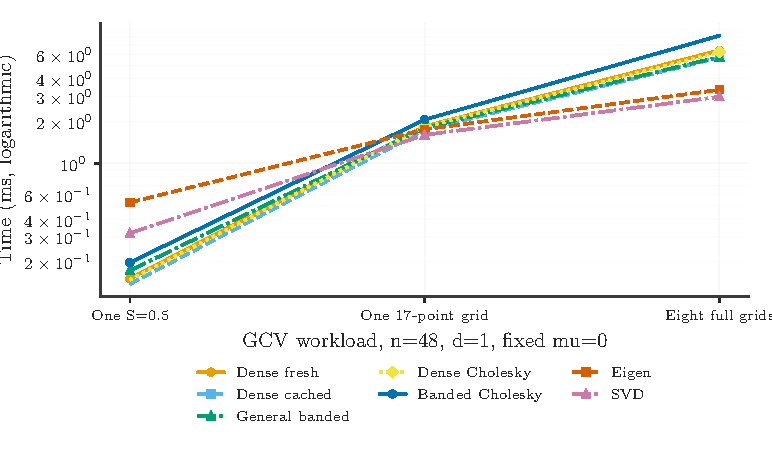
\includegraphics[width=.48\linewidth]{figures/windows_full_s_workloads.pdf}
\hfill
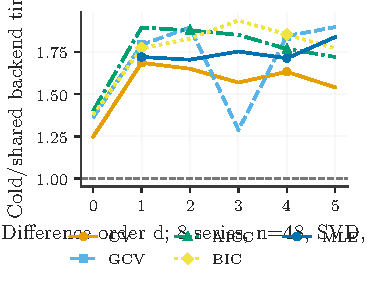
\includegraphics[width=.48\linewidth]{figures/windows_full_s_reuse_d.pdf}
\caption{Previously archived author-Windows
80,640-record study. Left: one scalar score,
one complete selection, and repeated searches
with backend-specific costs. Right: cold
versus shared preprocessing across
$d=0,\ldots,5$. The backends' validity
filters and exact sample settings are
provided in the reproducible archived
source; the two panels should not be
read as cross-hardware generalizations.}
\label{fig:expanded-workload-reuse}
\end{figure}

\begin{figure}[tbp]
\centering
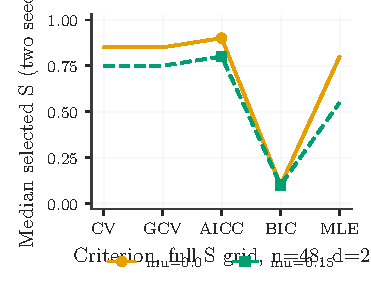
\includegraphics[width=.48\linewidth]{figures/windows_full_s_means.pdf}
\hfill
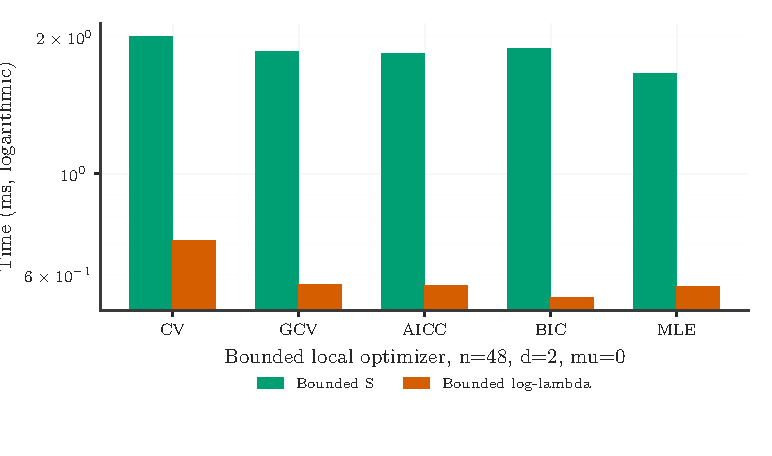
\includegraphics[width=.48\linewidth]{figures/windows_full_s_bounded.pdf}
\caption{Archived factorial comparisons:
left, selected $S$ across the five statistical
criteria under $\mu=0$ and $\mu=0.15$
for the matched candidate grid; right,
bounded \emph{local} searches over
$S$ versus $\log\lambda$.
These are separate inferential and
computational questions. A bounded
optimizer has no guaranteed global
minimum in either coordinate.}
\label{fig:expanded-mu-local}
\end{figure}

The same factorial records distinguish
seven numerical backends and all
difference orders; numerical failures
at extreme finite penalties were
screened \emph{before} a timing winner
was declared. This is particularly
important for higher order penalties:
an invalid fast dense solve does not
beat a slower accurate spectral
score. Full all-cell results, numerical
validity flags and reproducibility
metadata remain available for
inspection in the companion repository.

\subsection{Which backend is preferable for full trends?}
Table~\ref{tab:expanded-solver-orders}
reports seed-paired Windows measurements
for distinct difference orders,
a nonzero reference mean, and
several numbers of fitted curves.
These are actual full-trend timings,
not the score-only results above.
The 95\% intervals are \emph{pointwise}
bootstrap intervals; Holm-adjusted
$p$ values address the full predeclared
family of 63 solver-pair/workload
comparisons, rather than independent
tests chosen after observing the results.
Banded Cholesky is a distinct
specialized algorithm, not a new
name for the older general-banded solve.

\begin{table}[tbp]
\centering\footnotesize
\caption{Paired total-time ratio SVD/BChol
for archived full-trend computations:
ratio $>1$ favors banded Cholesky;
ratio $<1$ favors SVD. The interval is
seed-bootstrap pointwise 95\%;
Holm $p$ covers the complete
recorded family of comparisons.
$M$ is the number of fitted penalties.}
\label{tab:expanded-solver-orders}
\resizebox{\linewidth}{!}{\begin{tabular}{rrrrrll}
\toprule
$n$ & $d$ & $M$ & $\mu$ & SVD/BChol & 95\% pointwise CI & Holm $p$ \\
\midrule
96 & 1 & 16 & 0.00 & 2.205 & [2.193, 2.216] & 0.00315 \\
96 & 2 & 16 & 0.00 & 2.093 & [2.084, 2.101] & 0.00315 \\
96 & 2 & 16 & 0.15 & 2.103 & [2.097, 2.109] & 0.00315 \\
96 & 3 & 16 & 0.00 & 1.731 & [1.723, 1.742] & 0.00315 \\
96 & 5 & 16 & 0.00 & 1.168 & [1.163, 1.174] & 0.00315 \\
32 & 2 & 1 & 0.00 & 1.554 & [1.541, 1.568] & 0.00315 \\
32 & 2 & 64 & 0.00 & 0.419 & [0.417, 0.421] & 0.00315 \\
\bottomrule
\end{tabular}
}
\end{table}

\begin{figure}[tbp]
\centering
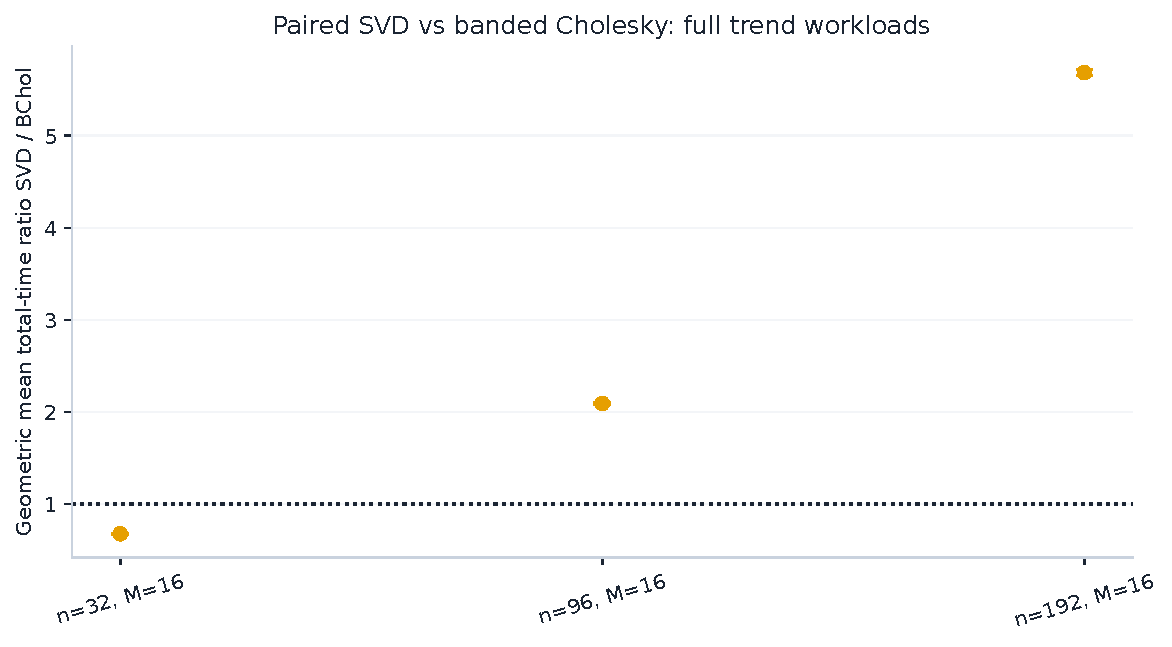
\includegraphics[width=.86\linewidth]{figures/final_solver_inference.pdf}
\caption{Archived seed-level paired time ratios
for selected full-curve workloads.
The dashed horizontal reference of one
denotes equal elapsed time, and the
intervals are pointwise, not simultaneous.
Neither a single backend nor a single
configuration is always preferred.}
\label{fig:expanded-paired-fig}
\end{figure}

The physical effect of reuse is central:
a prepared spectral transform makes
repeated $(\lambda,d)$ evaluations cheap,
while a specialized banded factorization
can avoid expensive dense preparation
for small numbers of full curves.
For example, the predeclared $d=2$
case at $n=32$ reverses its preferred
solver as the number of fitted
penalties grows from one to 64.
We do not extrapolate this crossover
to other numerical precision,
sample sizes or hardware.

\subsection{Accuracy before inversion speed}
The archived inversion results recorded
528 $(n,d,s,\text{method})$ case summaries
and no failures across their 35
technical repetitions per case.
This statement concerns precisely the
tested float64 targets and tolerances;
it does not guarantee success for every
representable $s$ or penalty spectrum.

\begin{table}[tbp]
\centering\footnotesize
\caption{Measured Brent, Newton, secant,
and bisection latency, iteration count,
failure count and maximum relative
smoothness-tail error for $n=120,d=2$
at $S=0.5$ and $S=0.99$.
All values are read from the author's
recorded float64 benchmark and require
a precomputed smoothness spectrum.
The analytic $d=0$ case is excluded.}
\label{tab:expanded-root}
\resizebox{\linewidth}{!}{\begin{tabular}{llrrrr}
\toprule
$S$ & Inversion method & Median $\mu$s & Fail / trials & Iterations & Max rel. tail error \\
\midrule
.5 & brentq & 91.50 & 0/35 & 10.0 & 1.8e-15 \\
.5 & newton & 88.30 & 0/35 & 5.0 & 2.2e-16 \\
.5 & secant & 157.70 & 0/35 & 24.0 & 1.1e-15 \\
.5 & bisect & 292.00 & 0/35 & 45.0 & 1.4e-13 \\
.99 & brentq & 93.70 & 0/35 & 11.0 & 3.3e-14 \\
.99 & newton & 118.60 & 0/35 & 8.0 & 0 \\
.99 & secant & 162.80 & 0/35 & 26.0 & 1.7e-13 \\
.99 & bisect & 282.00 & 0/35 & 45.0 & 7.7e-14 \\
\bottomrule
\end{tabular}
}
\end{table}

\begin{figure}[tbp]
\centering
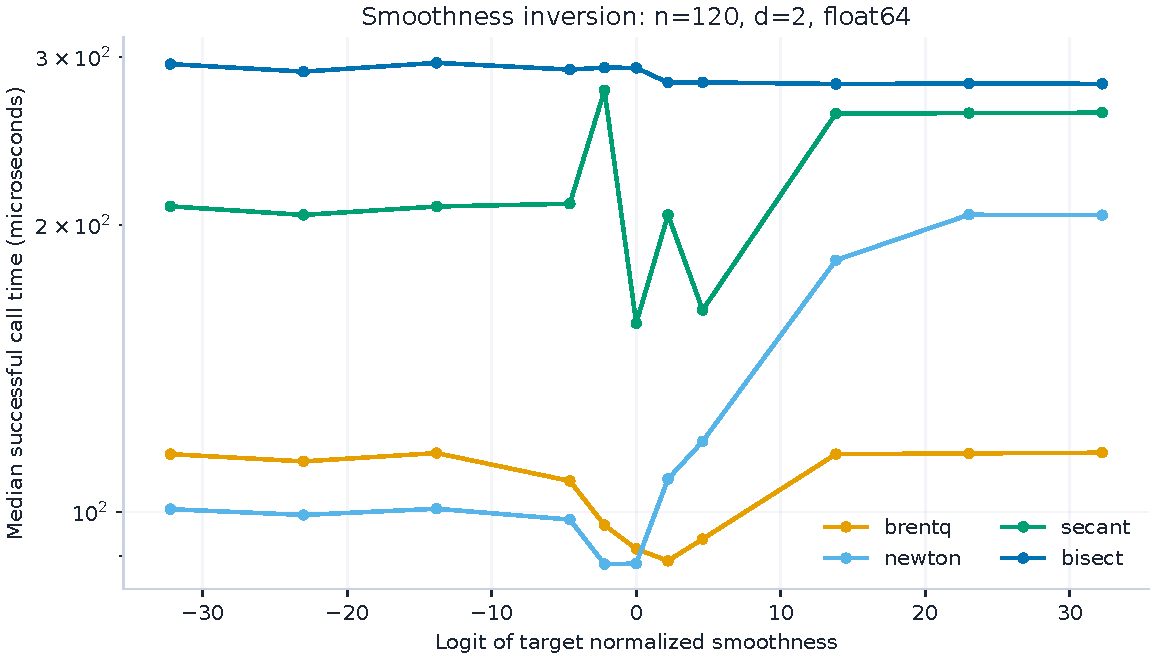
\includegraphics[width=.86\linewidth]{figures/final_inversion_speed.pdf}
\caption{Observed root inversion latencies
across $\operatorname{logit}(S)$ for
Brent, Newton, secant and bisection.
Missing or inaccurate solutions would
be explicitly recorded; only valid
outcomes contribute successful-call
medians. The plotted runtime excludes
initial spectral preprocessing.}
\label{fig:expanded-inverse-time}
\end{figure}

The distinction between full
search time and one inverse call
is important: root-finding is useful
for choosing a controlled target
but has a cost if repeated at
every candidate evaluation.
Cache a shared inverse grid
where reuse justifies it; do not
assume native-$S$ search is faster
than a numerical log-penalty search
simply because $S$ is easier to interpret.
